%%%%%%%%%%%%%%%%%%%%%%%%%%%
%% Document is an article for a4 paper
\documentclass[a4paper]{article}
%% Encoding is utf8
\usepackage[utf8]{inputenc}
%% Fonts
\usepackage[T1]{fontenc}
%% Include graphic.
\usepackage{graphicx}
%% Use PGF to draw.
\usepackage{tikz}
%% Use tabularx
\usepackage{tabularx}
\usepackage{multirow}
\usepackage{array}
%% Babel package
\usepackage[english]{babel}
%% Bit fields: to create message descriptions
\usepackage[bitheight=6ex]{bytefield}
%% Use hyper reference.
\usepackage[bookmarksopen=true]{hyperref}
\hypersetup{%
pdftitle={Share Resource},
pdfauthor={Anthony Jaguenaud},
pdfsubject={Share resource},
pdfkeywords={}}
%% Setup links.
\definecolor{darkred}{rgb}{0.5,0,0}
\definecolor{darkgreen}{rgb}{0,0.3,0}
\definecolor{darkblue}{rgb}{0,0,0.5}
\definecolor{darkbrown}{rgb}{0.28,0.07,0.07}

\hypersetup{%
  colorlinks=true,
  citecolor=darkblue,
  urlcolor=darkgreen,
  linkcolor=darkred,
  menucolor=darkbrown}

\newcommand{\field}[4]{
  \begin{tabular}{|p{3.5cm}|c|m{1cm}|m{2cm}|}
   \cline{1-1} \cline{3-4}
   #1 & \hspace{4cm} & #2 & #3 \\
   \hline
   \multicolumn{4}{|p{\textwidth}|}{#4} \\
   \hline
  \end{tabular}
}

\newcommand{\bitfield}[1]
{
    \begin{rightwordgroup}{Type\\\texttt{#1}}
      \wordbox{1}{\centering \texttt{#1}}
    \end{rightwordgroup} \\
}
\newcommand{\colorbitbox}[3]{%
\rlap{\bitbox{#2}{\color{#1}\rule{\width}{\height}}}%
\bitbox{#2}{#3}}

\newcommand{\SHABitboxes}{\bitbox{8}{[0]}
      \bitbox{8}{[1]}
      \bitbox{16}{\dots} \\
      \skippedwords \\
      \bitbox{16}{\dots}
      \bitbox{8}{[38]}
      \bitbox{8}{[39]}}

%\field{Header index}{Version}{Optional}{Header index is used to help to get information faster than reading fields one by one}
% \newcommand{\field}[4]{
%   \begin{tikzpicture}
%     \node (name) {#1};
%     \node (opt) {#2};
%     \node (version) [left = of opt] {#3};
%     \node (description) {#4};
%   \end{tikzpicture}
%
% }
% \newcommand{\field}[4]{
%   \begin{tabular}{|c|c|c|c|}
%   \cline{1-1}
%   #2 \\
%   \hline
%   \multirow{2}{*}{\rotatebox{90}{#1 }} & \multicolumn{3}{m{10cm}|}{#4} \\
%   \cline{2-4}
%   & \multicolumn{2}{c|}{#3} \\
%   \cline{1-3}
%   \end{tabular}
% }

\begin{document}
 \tableofcontents
 \section{Data format}
 \subsection{Directory and file organisation}
  \usetikzlibrary{trees}
\tikzstyle{every node}=[draw=black,thick,anchor=west]
\tikzstyle{selected}=[draw=red,fill=red!30]
\tikzstyle{optional}=[dashed,fill=gray!50]
\begin{tikzpicture}[%
  grow via three points={one child at (0.5,-0.7) and
  two children at (0.5,-0.7) and (0.5,-1.4)},
  edge from parent path={(\tikzparentnode.south) |- (\tikzchildnode.west)}]
  \node {root}
    child { node {04}
      child { node {\textbf{04}d528475b8f8dfb46107fc2fc98af2a2bc61ae1}}
    }
    child [missing] {}
    child { node {24}
      child { node {\textbf{24}80894a41445612d1cd7e1cb373598bd0500cc4}}
    }
    child [missing] {}
    child { node {40}
      child { node {\textbf{40}437af82bdcfa5122d6e592141b859888d07451}}
      child { node {\textbf{40}b69804e80e0192f041e964b0656d3ad8d3313e}}
    }
    child [missing] {}
    child [missing] {}
    child { node {6e}
      child { node {\textbf{6e}3be75e3b315c5a1ad32b23f76613b13e76aef9}}
    }
    child [missing] {}
    child { node {e6}
      child { node {\textbf{e6}3e3d1d2d7936278cab8d220dab6561db0c36e1}}
    }
    child [missing] {}
    child { node {fa}
      child { node {\textbf{fa}81dae4271daa04a584a77cf6ce721f42dd324d}}
    }
    child [missing] {}
    child { node {ff}
      child { node {\textbf{ff}085fda1d08567803896de7bb70b0dfc4b15383}}
    };

\end{tikzpicture}
\tikzstyle{every node}=[]

  Files are store in a directory.
Files represents Meta data storage units, or Data storage units.
Files are parts of a global resource.
We degign by “\emph{root}” directory the base directory use for storage.
The storage unit class, performs an SHA1 sum and set the name of the resource with this sum.
The first two characters of name are used to hash the files in \emph{root} directory.
The file name is not truncated in the subdirectory.
So, the first two characters of files in a subdirectory are the same for all files.
\\
\begin{tabular}{|c|m{4cm}|c|}
 \hline
 {Variable} & {\centering Description} & {Default value} \\
 \hline
 \emph{Root} & Root directory of storage units. & $\sim$/.local/share/CapProject/shareLib/ \\
 \hline
\end{tabular}

 \subsection{Meta Units format}
  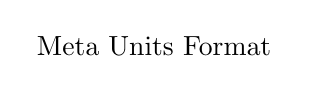
\begin{tikzpicture}
 \path (1,1) node{Meta Units Format};
\end{tikzpicture}


  Meta unit file format have a particular format.
This file does not contain data, it contains the list of all data file units used for a resource, the resource id, and others informations detailed below.
The first bytes of the file contain \emph{RS-META}\footnote{This is a 0 string terminated. So there are 8 characters reserved.}.
Then start real contain.
See Figure~\ref{fig:META-FILE-FORMAT} for more detail.
The next 8 bytes are the same than 8 first.
\begin{itemize}
 \item If the bytes in range [8..15] are not the same than in range [0..7] that means file is encrypted.
The key is not store by Share Resource library.
User software must delegate a key and the library will search the meta units that unlock.
The key is a symetric key.
 \item If the bytes in range [8..15] are the same than in range [0..7] that means unit is not encrypted.
\end{itemize}
\begin{figure}[htbp]
  \centering
\begin{bytefield}[bitwidth=2em]{16}
    \bitheader{0,7-8,15} \\

    \begin{rightwordgroup}{file header}
      % We have to do the \parbox explicitly in the next line because
      % \hyperlink typesets its argument in horizontal mode.\parbox{\width}{}
      \bitbox{1}{R} &
      \bitbox{1}{S} &
      \bitbox{1}{-} &
      \bitbox{1}{M} &
      \bitbox{1}{E} &
      \bitbox{1}{T} &
      \bitbox{1}{A} &
      \bitbox{1}{\textbackslash 0} &
      \bitbox{1}{R} &
      \bitbox{1}{S} &
      \bitbox{1}{-} &
      \bitbox{1}{M} &
      \bitbox{1}{E} &
      \bitbox{1}{T} &
      \bitbox{1}{A} &
      \bitbox{1}{\textbackslash 0}
   \end{rightwordgroup} \\

  \begin{rightwordgroup}{Meta data}
    \wordbox{2}{First meta field object} \\
    \wordbox[lrt]{1}{%
      \parbox{0.6\width}{\centering (Meta field objects)}} \\
    \skippedwords \\
    \wordbox{2}{Last meta field object}
  \end{rightwordgroup}
  \end{bytefield}
  \caption{META file format.}
  \label{fig:META-FILE-FORMAT}
  \end{figure}




Data in the \emph{META unit} are serialized\footnote{That means that data can be stored with no order. As the \hyperlink{fields:header-index}{header index} is not to be sure to be in the first place.}.

Each field have the same scheme (Figure~\ref{fig:META-FIELD-FORMAT}):

\begin{figure}[htbp]
  \centering
\begin{bytefield}{32}
    \bitheader{0,7-8,15-16,23-24,31} \\

    \begin{rightwordgroup}{header}
      % We have to do the \parbox explicitly in the next line because
      % \hyperlink typesets its argument in horizontal mode.\parbox{\width}{}
      \wordbox{1}{\hyperlink{META-FIELD-Size}{\centering Size}} \\
      \wordbox{1}{\hyperlink{META-FIELD-Type}{type}}
    \end{rightwordgroup} \\

  \begin{rightwordgroup}{Object}
    \wordbox[lrt]{1}{%
      \parbox{0.6\width}{\centering (Object contain.)}} \\
    \skippedwords \\
    \wordbox[lrb]{1}{}
  \end{rightwordgroup}
  \end{bytefield}
  \caption{META object field.}
  \label{fig:META-FIELD-FORMAT}
  \end{figure}


  \begin{itemize}
   \item \hypertarget{META-FIELD-Size}{Size} of the object in byte. This include header, for a nul size object the size is 8.
   \item \hypertarget{META-FIELD-Type}{Type} of the object. Can be \emph{ResourceId} for example.
          All types are listed at the \hyperlink{META-FIELD-All-Types}{here}.
  \end{itemize}





The list of fields are in table \ref{tab:field-list}.

\begin{table}[htbp]
  \begin{tabular}{l|c|c|c}
    Name & introduce version & obsolete version & last version \\
    \hline
    \hyperlink{fields:meta-version}{Meta version} & 0.1 & & \\
    \hyperlink{fields:header-index}{Header index} & 0.1 & & \\
    \hyperlink{fields:resource-id}{Resource Id} & 0.1 & & \\
    \hyperlink{fields:resource-name}{Resource Name} & 0.1 & & \\
    \hyperlink{fields:data-index}{Data index} & 0.1 & & \\
    \hyperlink{fields:data-file}{Data file} & 0.1 & & \\
    \hyperlink{fields:auth-user-index}{Authorized users index} & 0.1 & & \\
    \hyperlink{fields:auth-user}{Authorized user} & 0.1 & & \\
    \hyperlink{fields:version}{Resource version} & 0.1 & & \\
    \hyperlink{fields:parents}{Parent} & 0.1 & & \\
  \end{tabular}
  \caption{List of fields in Meta File}
  \label{tab:field-list}
\end{table}


\hypertarget{fields:meta-version}{\subsubsection{Meta version}}
\field{Meta version}{v0.1}{Mandatory}{Meta version field is the version of the file format. For example, v0.1 means that meta file respects the 0.1 file format.}

This is the field that define the version format of meta file. This field is mandatory, and it should be the first field of file.

\begin{figure}[htbp]
  \centering
  \begin{bytefield}{32}
    \bitheader{0,7-8,15-16,23-24,31} \\

    \begin{rightwordgroup}{Size}
      % We have to do the \parbox explicitly in the next line because
      % \hyperlink typesets its argument in horizontal mode.\parbox{\width}{}
      \wordbox{1}{\centering 12}
    \end{rightwordgroup} \\
    \bitfield{0x00010001}

    \begin{rightwordgroup}{Version}
      \bitbox{16}{Main version}
      \bitbox{8}{Minor version}
      \bitbox{8}{Maintenance version}
    \end{rightwordgroup}
  \end{bytefield}
  \caption{META version field.}
  \label{fig:FIELD:meta-version}
\end{figure}

The figure \ref{fig:FIELD:meta-version} describes the object.
First field is the size of object and its value is 12.
Second field is the type of object, the type of this object is: \texttt{0x00010001}.
Third field is the version of the file format.
Main version is the main version of compatible software.
Major version is the major number of compatible software.
Maintenance version is the bugfix version of a delivered version.

The values change only if file format change.
The version 0.2.1 of software can have a 0.1.0 file format version.

Ex: The software 0.4.5 have a file format version: 0.3.1.
Message is visible on figure \ref{fig:FIELD:meta-version:example}
\begin{figure}[htbp]
  \centering
  \begin{bytefield}{32}
    \bitheader{0,7-8,15-16,23-24,31} \\

    \begin{rightwordgroup}{Size}
      % We have to do the \parbox explicitly in the next line because
      % \hyperlink typesets its argument in horizontal mode.\parbox{\width}{}
      \wordbox{1}{\centering 12}
    \end{rightwordgroup} \\
    \bitfield{0x00010001}

    \begin{rightwordgroup}{Version}
      \bitbox{16}{0}
      \bitbox{8}{3}
      \bitbox{8}{1}
    \end{rightwordgroup}
  \end{bytefield}
  \caption{META version field example.}
  \label{fig:FIELD:meta-version:example}
\end{figure}

\hypertarget{fields:header-index}{\subsubsection{Header index}}
\field{Header index}{v0.1}{Optional}{Header index is used to help to get information faster than reading fields one by one}

This index is used to create an rapid acces to main informations.
This main index reference others index.
The order of informations are important.
The figure \ref{fig:FIELD:header-index} describes the format.

\begin{figure}[htbp]
  \centering
  \begin{bytefield}{32}
    \bitheader{0,7-8,15-16,23-24,31} \\

    \begin{rightwordgroup}{Size}
      % We have to do the \parbox explicitly in the next line because
      % \hyperlink typesets its argument in horizontal mode.\parbox{\width}{}
      \wordbox{1}{\centering 20}
    \end{rightwordgroup} \\
    \bitfield{0x00010002}

    \begin{rightwordgroup}{Resource Id}
      \wordbox{1}{offset of \hyperlink{fields:resource-id}{Resource Id}}
    \end{rightwordgroup}\\
    \begin{rightwordgroup}{Users index}
      \wordbox{1}{offset of \hyperlink{fields:auth-user-index}{Users index}}
    \end{rightwordgroup}\\
    \begin{rightwordgroup}{Resource Id}
      \wordbox{1}{offset of \hyperlink{fields:data-index}{Data index}}
    \end{rightwordgroup}\\
  \end{bytefield}
  \caption{META Header index.}
  \label{fig:FIELD:header-index}
\end{figure}


\hypertarget{fields:resource-id}{\subsubsection{Resource Id}}
\field{Resource Id}{v0.1}{Mandatory}{Resource Id is the Id of the resource. This Id is a uniq Id to get resource. By default Id is the initial Id SHA1 of initial Resource.}

\hypertarget{fields:resource-name}{\subsubsection{Resource Name}}
\field{Resource Name}{v0.1}{Optional}{The name of a resource. This name can be used to retreive a resource from its name.}

\hypertarget{fields:data-index}{\subsubsection{Data index}}
\field{Data index}{v0.1}{Optional}{List all \hyperlink{fields:data-file}{Data files fields} use for store the resource.}

\hypertarget{fields:data-file}{\subsubsection{Data File}}
\field{Data file}{v0.1}{Mandatory}{This field is used to retreive the file cache of a part of the resource.}

\hypertarget{fields:auth-user-index}{\subsubsection{Authorized users index}}
\field{Authorized users index}{v0.1}{Optional}{This index is used to store all authorized user.}

\hypertarget{fields:auth-user}{\subsubsection{Authorized user}}
\field{Authorized user}{v0.1}{Mandatory}{This field define a user. This field is encrypted only corresponding user can read the field. The key for encrypted fields is stored encrypted with the public key of user.}

\hypertarget{fields:version}{\subsubsection{Resource version}}
\field{Resource version}{v0.1}{Mandatory}{This field is used to follow changes in a resource. Detect that current version is obsolete.}

\hypertarget{fields:parents}{\subsubsection{Parent}}
\field{Parent}{v0.1}{Mandatory}{This field determines the previous version of the resource. There can be various parents in case of merge.}






 \subsection{Data Units format}
  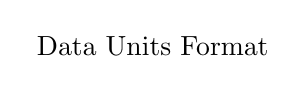
\begin{tikzpicture}
 \path (1,1) node{Data Units Format};
\end{tikzpicture}


  The data are store in data unit. The format of these units is composed with a header, data and a footer.
Detail are in figure~\ref{fig:DATA-FILE-FORMAT}~:
\begin{figure}[htbp]
  \centering
\begin{bytefield}[bitwidth=2em]{16}
    \bitheader{0,7-8,15} \\

    \begin{rightwordgroup}{file header}
      % We have to do the \parbox explicitly in the next line because
      % \hyperlink typesets its argument in horizontal mode.\parbox{\width}{}
      \wordbox{2}{Resource ID}
   \end{rightwordgroup} \\

  \begin{rightwordgroup}{Data\\\emph{encrypted}}
    \wordbox{5}{%
      \parbox{0.6\width}{\centering (DATA)}}
  \end{rightwordgroup} \\
  \begin{rightwordgroup}{Footer\\\emph{encrypted}}
    \wordbox{2}{SHA1 of DATA}
  \end{rightwordgroup} \\

  \end{bytefield}
  \caption{DATA file format.}
  \label{fig:DATA-FILE-FORMAT}
\end{figure}

The first field is the resource id. With this field, we can retreive the META files of resource.
Data part is data array sent by software. The SHA1 is the SHA1 of data. The parts DATA and footer can be encrypted depending of META files.

\end{document}
